\begin{frame}{Fake estimation dileptau}
    \begin{figure}
        \centering
        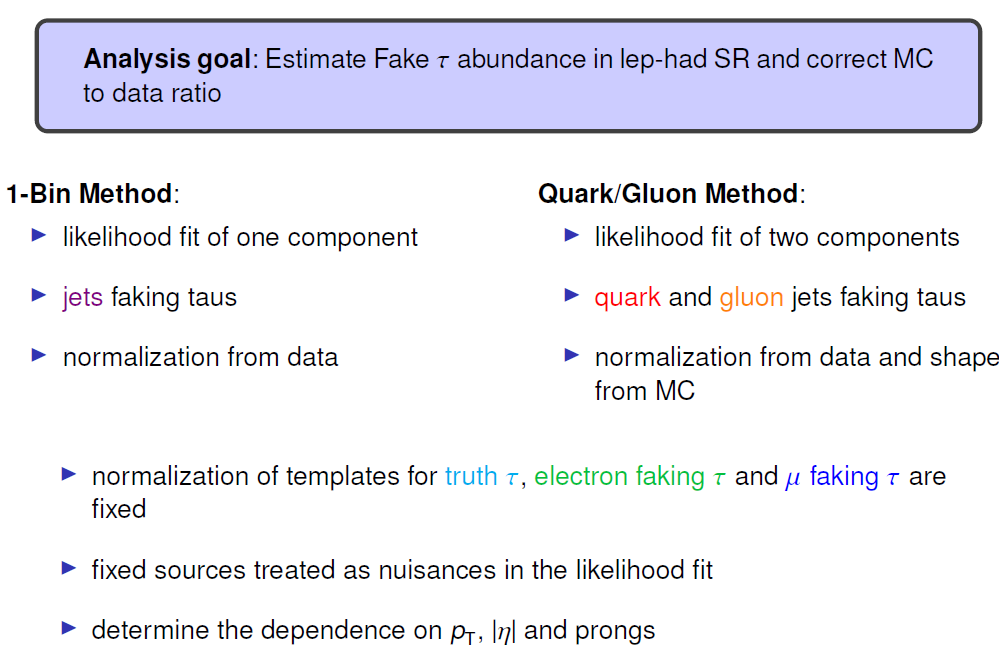
\includegraphics[width=\textwidth]{fake_strategy}
    \end{figure}
\end{frame}
 
\begin{frame}{One bin method dileptau Control Region}
    \begin{figure}
        \centering
        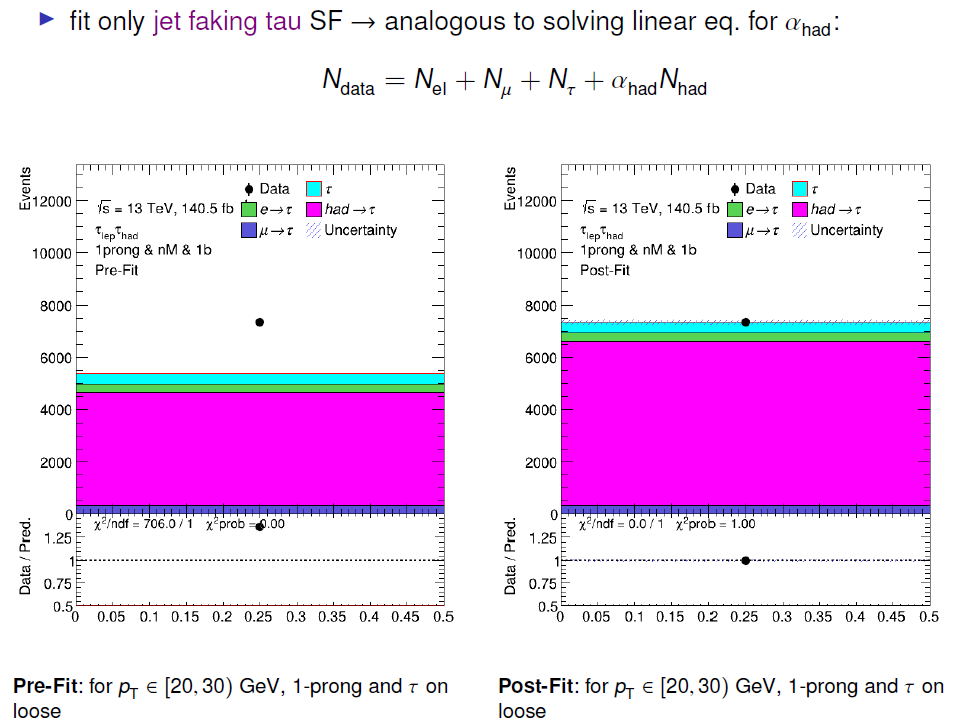
\includegraphics[width=0.85\textwidth]{oneBinCR}
    \end{figure}
\end{frame}

\begin{frame}{One bin method dileptau Signal Region}
    \begin{figure}
        \centering
        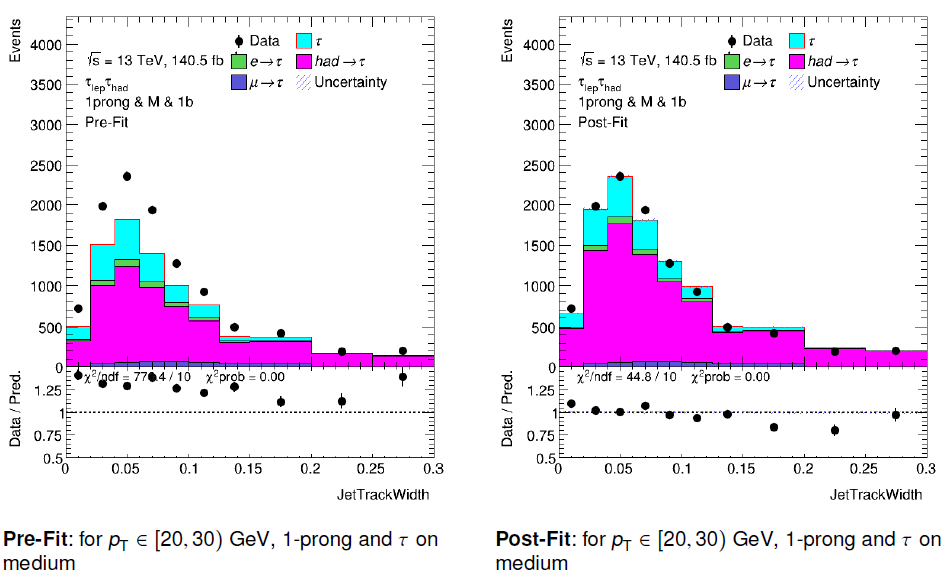
\includegraphics[width=0.85\textwidth]{oneBinSR}
    \end{figure}
\end{frame}

\begin{frame}{Quark/gluon method dileptau Control Region}
    \begin{figure}
        \centering
        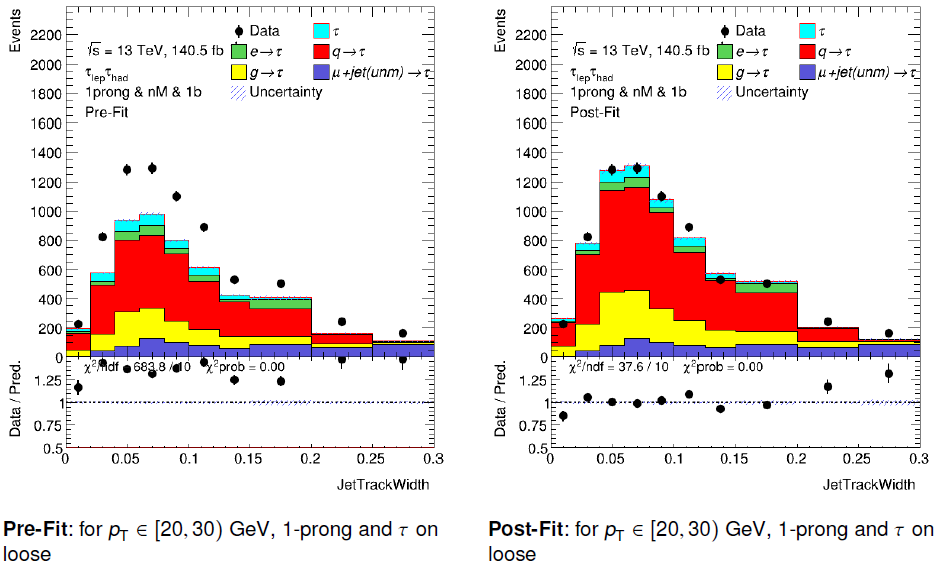
\includegraphics[width=0.95\textwidth]{quarkGluonCR}
    \end{figure}
\end{frame}

\begin{frame}{Quark/gluon method dileptau Signal Region}
    \begin{figure}
        \centering
        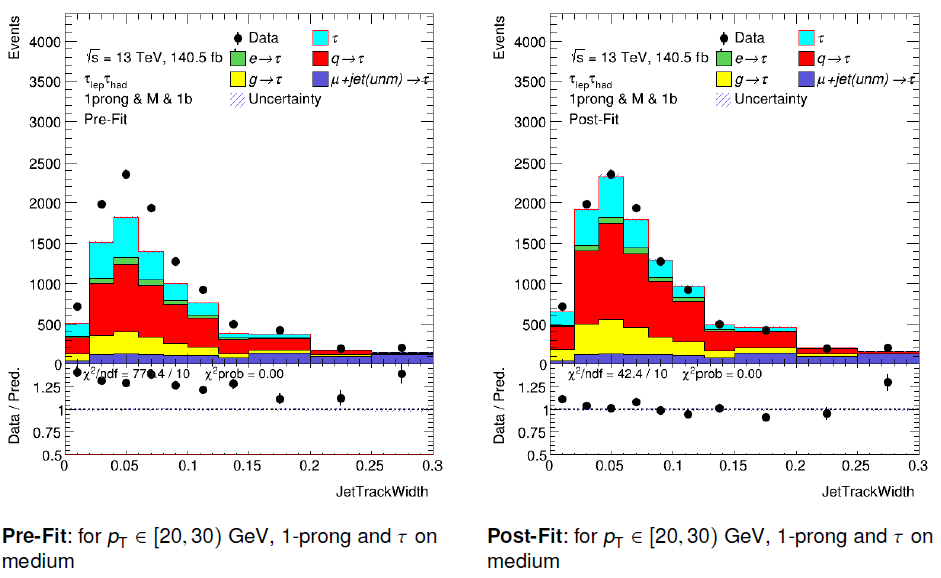
\includegraphics[width=0.95\textwidth]{quarkGluonSR}
    \end{figure}
\end{frame}

\begin{frame}{Fake Estimation Lepditau}
    \begin{itemize}
        \item Using template fit method
    \end{itemize}
    \begin{columns}
        \begin{column}{0.5\textwidth}
            \begin{figure}
                \centering
                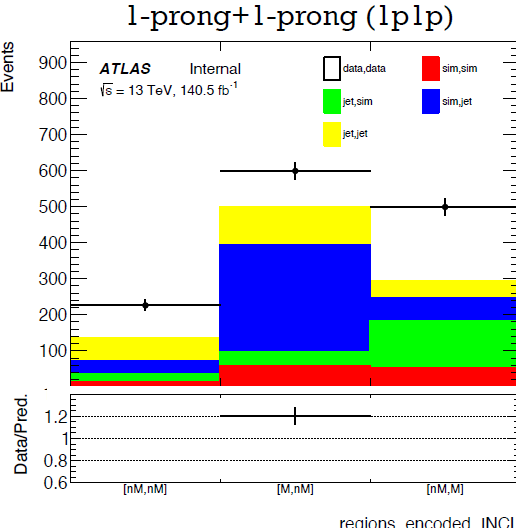
\includegraphics[width=\textwidth]{oleh_1}
            \end{figure}
        \end{column}
        \begin{column}{0.5\textwidth}
            \begin{figure}
                \centering
                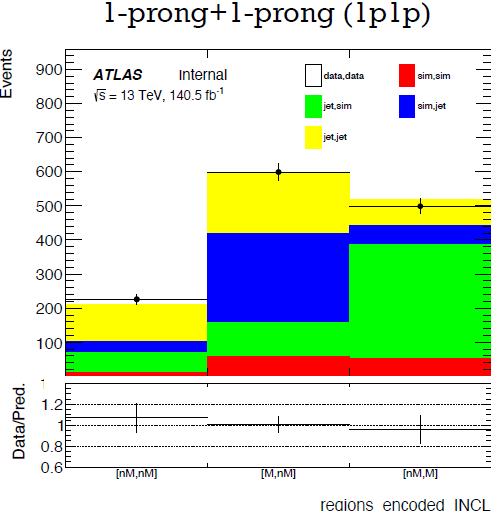
\includegraphics[width=\textwidth]{oleh_2}
            \end{figure}
        \end{column}
    \end{columns}
\end{frame}

\begin{frame}{Lepditau fake estimation fit results}
    \begin{figure}
        \centering
        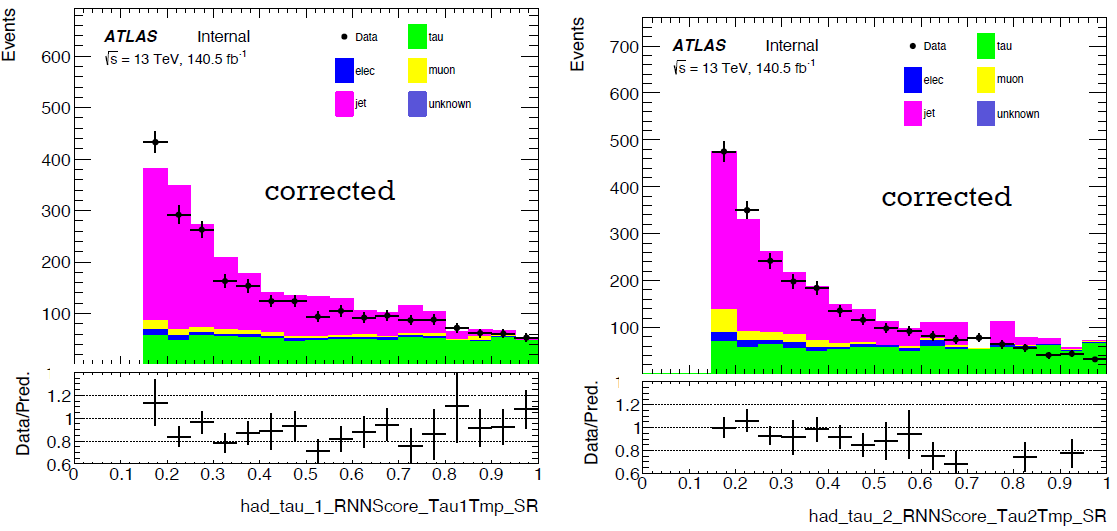
\includegraphics[width=\textwidth]{oleh_3}
    \end{figure}
\end{frame}

\begin{frame}{Lepditau fake estimation fit results}
    \begin{figure}
        \centering
        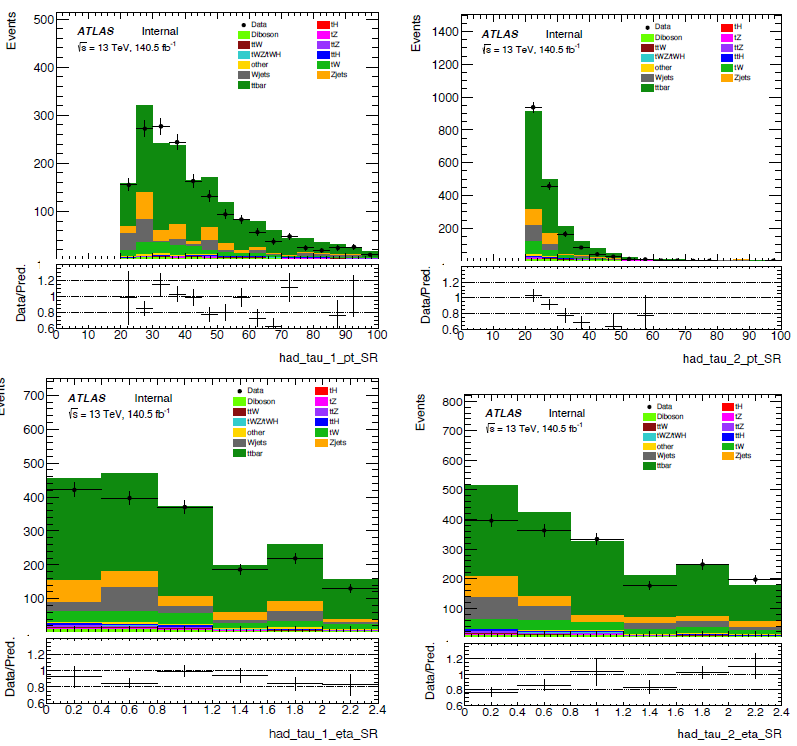
\includegraphics[width=0.74\textwidth]{oleh_4}
    \end{figure}
\end{frame}

\begin{frame}{Lepton Assigment Method}
    \begin{itemize}
        \item Establish method for lepton assignment
        \vspace{0.6cm}
        \item Tested promising variables for assignment
        \vspace{0.6cm}
        \item $m_{pred,t}(lep(Higgs)) - m_{pred,t}(lep(top)) > 0$
        \vspace{0.6cm}
        \item Generality allows to expand to SS events
    \end{itemize}
\end{frame}

\begin{frame}{Lepton Assigment Results}
    \begin{figure}
        \centering
        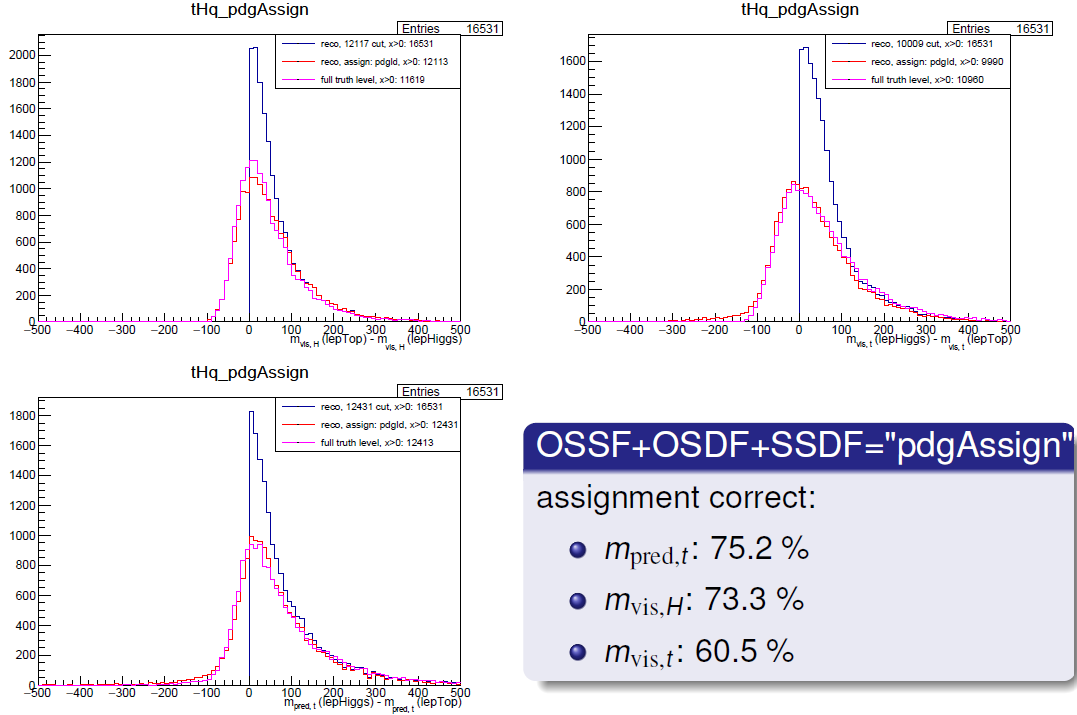
\includegraphics[width=0.9\textwidth]{assignment_results}
    \end{figure}
\end{frame}
